\chapter{De Galileitransformatie}
\vspace{-1cm}\begin{flushright}
{\it `Philosophy is written in this grand book \\-I mean the
  Universe-\\it is written in the language of mathematics.'}\\
 G. Galilei\end{flushright}
Gebeurtenissen spelen zich af op zekere plaatsen en tijdstippen.
Een plaats beschrijven we t.o.v. een co\"{o}rdinatenstelsel en tijd meten we 
met een klok.

% \begin{figure}[h]
% \begin{center}
% \mbox{\epsfxsize=10cm\epsffile{syllabus.pictures/xyzr.eps}}
% \caption{Driedimensionaal, orthogonaal co\"{o}rdinatenstelsel}
% \label{f:galilei1}
% \end{center}
% \end{figure}

\section{Co\"ordinatenstelsel}
Het is duidelijk dat de keuze van een specifiek co\"ordinatenstelsel,
ten opzichte waarvan beweging wordt beschreven, geheel vrij is. Het
verdient natuurlijk de voorkeur een co\"ordinatenstelsel te kiezen
waarin de beschrijving van beweging het gemakkelijkst is. De
bewegingen van de conducteur op een trein bijvoorbeeld, worden het
makkelijkst beschreven in een stelsel waarin de trein zelf
stilstaat. De eenparige beweging van de trein ten opzichte van
een co\"ordinatenstelsel verbonden met de aarde wordt (in het ideale
geval) tenslotte niet eens opgemerkt.


\begin{figure}[ht]
\centering
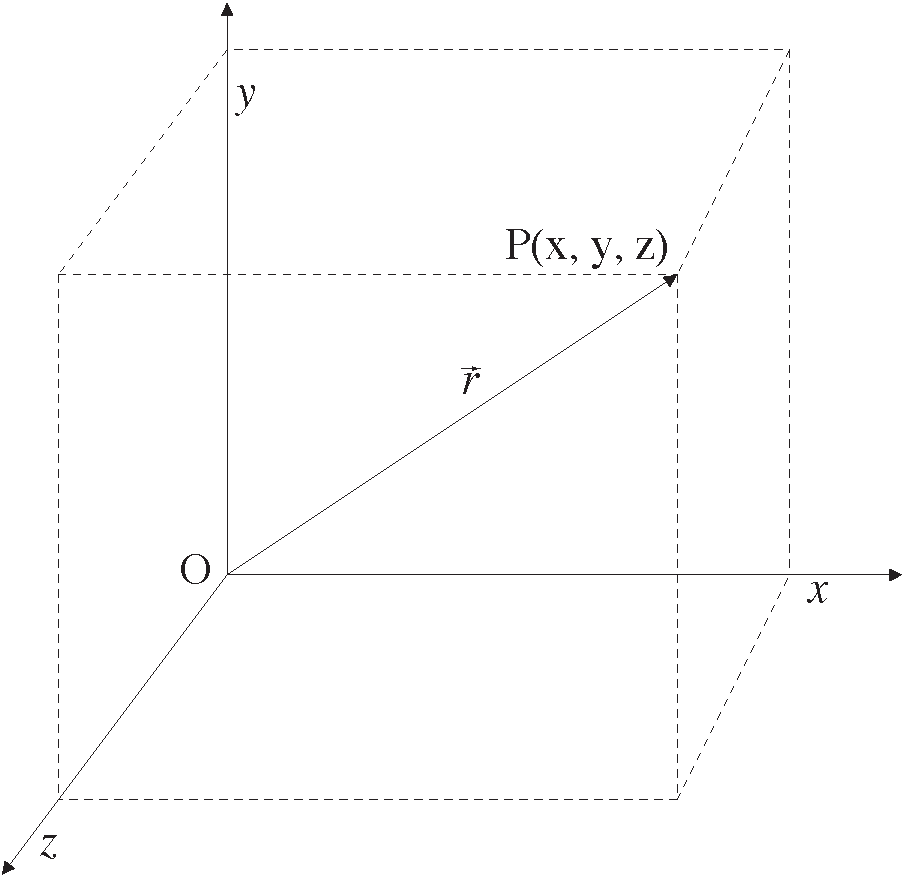
\epsfig{file=xyzr.pdf, width=0.5\textwidth}
\caption{{\sl Driedimensionaal, orthogonaal co\"{o}rdinatenstelsel}}
\label{f:galilei1}
\end{figure}


In figuur~\ref{f:galilei1} is een rechtshandig, orthogonaal,
driedimensionaal co\"{o}rdina-tenstelsel weergegeven.  Een vector
$\vec{r}$ wijst vanuit de oorsprong ${\cal O}$ naar een punt waarvan
de positie door drie getallen, de co\"{o}rdinaten, $x, y$ en $z$ wordt
aangegeven.  (Cartesiaanse co\"ordinaten). Orthogonaal wil zeggen dat de
drie assen loodrecht op elkaar staan.  Rechtshandig wil zeggen dat als
we langs de positieve $z$-as kijken, we de positieve $x$-as naar de
positieve $y$-as roteren met een rechtshandige draai\footnote{Of
bekijk het assenstelsel met uw handen: de positieve $x$-as uw duim, de
$y$-as de wijsvinger en de $z$-as de middelvinger.}.

Natuurlijk kunnen ook andere definities voor de co\"ordinaten gekozen
worden, bijvoorbeeld twee hoeken $\theta$ en $\phi$ ten opzichte van de assen en de
lengte van de vector, $r$ (bolco\"ordinaten). Meer specifiek: de 
poolhoek $\theta$ correspondeert met de hoek tussen de vector en de
$z$-as, de azimuth hoek $\phi$ is de openingshoek met de $x$-as, na projectie van de vector in het $x-y$ vlak.
Deze bolco\"ordinaten kunnen in  Cartesiaanse co\"ordinaten worden getransformeerd via
\begin{eqnarray}
x & = & r \sin \theta \cos \phi \\
y & = & r \sin \theta \sin \phi \\
z & = & r \cos \theta
\end{eqnarray}

Ongeacht de definitie van de co\"ordinaten, zullen er altijd {\em
drie} nodig zijn om een punt te bepalen in de ruimte. Dit is de
essentie van een drie-dimensionale ruimte. We zullen in dit college
verder alleen Cartesiaanse co\"ordinatenstelsels beschouwen. Als notatie 
van een drie-dimensionale vector, $\vec{x}$, gebruiken we een pijltje boven de symboolnaam. De componenten van 
een vector $\vec{x}$ geven we aan met de labels $(x,y,z)$.

Beschouw nu twee Cartesische co\"ordinaatsystemen, met label $S$ en
$S'$, die verschoven en geroteerd zijn ten opzichte van elkaar. Bekijk het geval dat ze 
beide hetzelfde punt in de ruimte beschrijven. In het ene stelsel,
$S$, heeft het punt $\vec{p}$ de co\"ordinaten $(p_x,p_y,p_z)$. Hetzelfde punt beschreven door het andere stelsel $S'$, heet nu $\vec{p}'$ en heeft de co\"ordinaten $(p'_x, p'_y,
p'_z)$. Met andere woorden, de waarden van de co\"ordinaten hangen
af van de keuze van het co\"ordinaatenstelsel. Dit geldt niet voor de
{\sl afstand} tussen twee punten in de ruimte. Deze afstand is
onafhankelijk van de keuze van de oorsprong en rotatie van het co\"ordinaatenstelsel, en wordt
daarom een {\sl invariante} grootheid genoemd. De afstand $\Delta r$ tussen twee
punten $\vec{x}_1$ en $\vec{x}_2$ in Cartesiaanse co\"ordinaten kan
verkregen worden met
\[
\Delta r = \sqrt{ (x_2-x_1)^2+(y_2-y_1)^2+(z_2-z_1)^2 }.
\]
oftewel
\[
(\Delta r)^2 = (\Delta x)^2 + (\Delta y)^2 + (\Delta z)^2
\]
De waarde van deze afstand $\Delta r$ hangt natuurlijk wel van de keuze van
de eenheden af.


% \begin{figure}[h]
% \begin{center}
% \mbox{\epsfxsize=8cm\epsffile{syllabus.pictures/systems.eps}}
% \caption{Tweedimensionaal, orthogonaal co\"{o}rdinatenstelsel $S'$ beweegt
% met constante snelheid $v$ t.o.v. co\"{o}rdinatenstelsel $S$}
% \label{f:galilei2}
% \end{center}
% \end{figure}

\begin{figure}[ht]
\centering
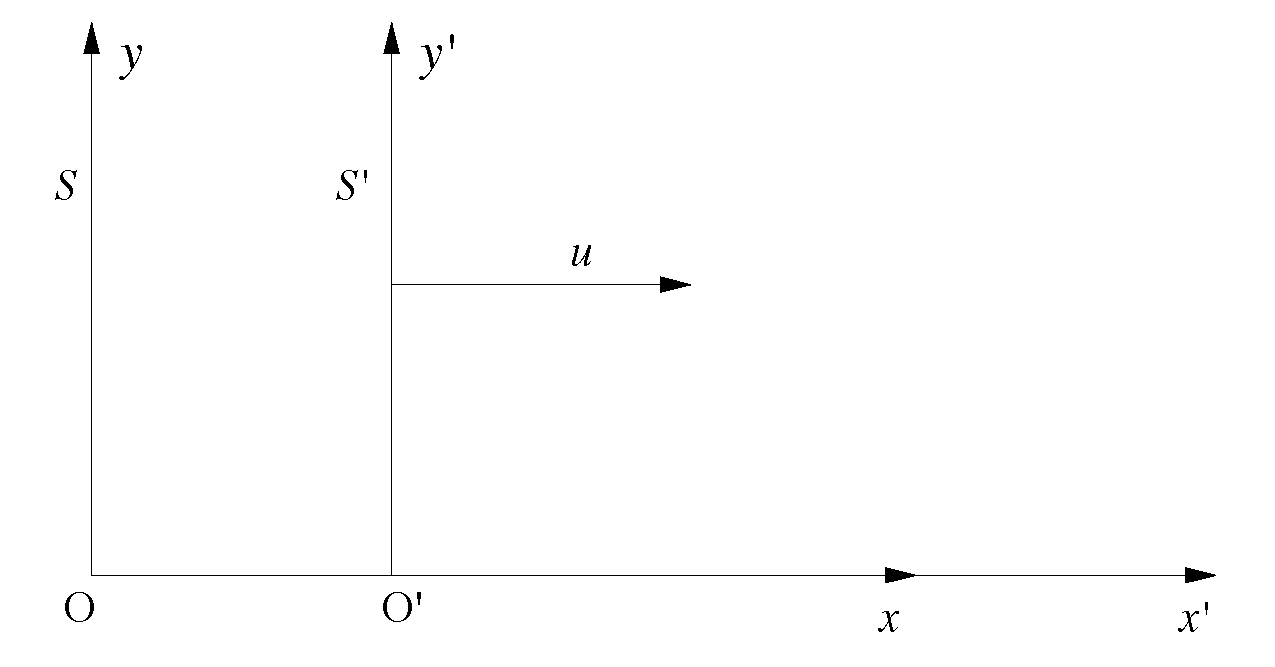
\epsfig{file=systems.pdf, width=0.7\textwidth}
\caption{{\sl Tweedimensionaal, orthogonaal co\"{o}rdinatenstelsel $S'$ beweegt
met constante snelheid $v$ t.o.v. co\"{o}rdinatenstelsel $S$}}
\label{f:galilei2}
\end{figure}

Indien we verschijnselen beschrijven die zich in een plat vlak afspelen 
is een tweedimensionaal co\"{o}rdinatenstelsel voldoende, en een punt
in het platte vlak wordt met twee co\"ordinaten beschreven.
In figuur~\ref{f:galilei2} is een tweedimensionaal co\"{o}rdinatenstelsel $S$ 
getekend en een tweedimensionaal co\"{o}rdinaten-stelsel $S^{'}$ dat met 
constante snelheid $v$ beweegt t.o.v. $S$, in de $x$-richting. Denk
bijvoorbeeld aan een trein bij het station, waarbij stelsel $S$ met
het perron correspondeert, en stelsel $S'$ met de rijdende trein.

We vragen ons nu af hoe we co\"{o}rdinaten (van bijvoorbeeld de baan van 
een puntmassa) gemeten t.o.v. $S$ kunnen uitdrukken in de co\"{o}rdinaten 
(van het zelfde verschijnsel) gemeten t.o.v. $S^{'}$.
Het antwoord kan gemakkelijk worden verkregen:
\begin{eqnarray}
\label{v:galilei1a}
y' &=& y\\
\label{v:galilei1b}
x' &= & x - vt
\end{eqnarray}
waar $t$ de tijd voorstelt (als beginvoorwaarde hebben we gekozen dat op tijd $t=0$ de co\"{o}rdinatenstelsels $S$ en $S^{'}$ samenvallen).

De {\sl snelheid} in de $x$-richting is per definitie de afgeleide 
van de $x$-co\"{o}rdinaat naar de tijd:
\begin{eqnarray*}
V_{x} & \equiv & \frac{dx(t)}{dt}
\end{eqnarray*}
Ten opzichte van $S^{'}$ geldt:
\begin{eqnarray*}
V_{x}^{'} & = &  \frac{dx^{'}}{dt}
\end{eqnarray*}
en dus volgt
\begin{equation}
\label{v:galilei2}
V_{x}^{'} = V_{x} -v
\end{equation}
We hebben als vanzelfsprekend aangenomen dat
\begin{eqnarray*}
t^{'} & = &  t
\end{eqnarray*}
d.w.z. we hebben aangenomen dat de tijd in $S^{'}$ en $S$ op identieke wijze 
verloopt.
Het zal in de loop van dit college blijken dat we deze `vanzelfsprekendheid'
moeten herzien!

Formules~\ref{v:galilei1a} en \ref{v:galilei1b} zijn overigens ook
volstrekt voor de hand liggend (en zoals we in de inleiding al zagen, moeten
herzien): als een fietser zich met snelheid $V_{x}$ over een weg
beweegt (stelsel $S$) en een voetganger (stelsel $S{'}$) zich met een
snelheid $v$ in dezelfde richting over die weg beweegt, dan beweegt de
fietser t.o.v. de voetganger met snelheid $V_{x}^{'} = V_{x} -
v$. Gaan fietser en voetganger even hard, d.w.z. $V_{x} = v$, dan is
hun relatieve snelheid $V_{x}^{'} = 0$. D\'{i}t resultaat zullen we
niet hoeven te herzien!

De {\sl versnelling} is per definitie de afgeleide van de snelheid 
naar de tijd :
\begin{eqnarray*}
a_{x} & \equiv & \frac{dV_{x}}{dt}
\end{eqnarray*}
Omdat $v$ constant is is nu gemakkelijk na te gaan dat:
\begin{equation}
\label{v:galilei3}
a_{x}^{'}  = a_{x}
\end{equation}
Versnellingen, en dus krachten ($\vec{F} = m\vec{a}$), zijn dus gelijk
in $S$ en $S^{'}$.  Meer in het algemeen blijkt dat de wetten van de
mechanica er hetzelfde uitzien in $S$ en $S^{'}$.  Als we hier even
over nadenken is dit een heel bevredigend en gewenst resultaat.  Het
zou een onaantrekkelijk idee zijn dat de natuurwetten zouden afhangen
van de `toevallige' bewegingstoestand van de natuurkundige die deze
wetten opspoort.

Formules~\ref{v:galilei1a} en~\ref{v:galilei1b} staan bekend als de
\textit{Galileitransformatie}.  Met behulp van deze formules kunnen we dus
co\"{o}rdinaten gemeten in het ene co\"{o}rdinatenstelsel,
{\sl transformeren} naar co\"{o}rdinaten in het andere
co\"{o}rdinaten-stelsel.  Wiskundig gezien is deze transformatie heel
eenvoudig, maar natuurkundig gezien is de observatie dat de wetten van
de mechanica hun vorm behouden (`gelijk blijven') van diepgaande
betekenis.  We zouden het als volgt kunnen formuleren: natuurkundig
gezien zijn alle co\"{o}rdinatenstelsels\footnote{We beperken ons in
dit college tot co\"{o}rdinatenstelsels die met constante snelheid (eenparig) ten
opzichte van elkaar bewegen. Co\"ordinaatstelsels die ook
versnellingen t.o.v. elkaar ondergaan worden behandeld in Einsteins
`Algemene Relativiteitstheorie'.} equivalent.  Of nog anders: er is geen
co\"{o}rdinatenstelsel dat onze voorkeur verdient.  

In het voorbeeld van het perron en de rijdende trein betekent dit het
volgende. Indien twee waarnemers ten opzichte van elkaar
eenparig rechtlijnig bewegen (een waarnemer op perron, de ander in de
trein), zullen ze precies dezelfde fysische verschijnselen
meten. Voorwerpen kunnen worden gedraaid en verschoven; hun meetkundige
eigenschappen zijn gelijk. En een voorwerp dat aan zichzelf wordt
overgelaten, d.w.z. waarop geen krachten werken, blijft in rust of beweegt
zich eenparig rechtlijnig. Dit is de definitie van een {\em
  inertiaalsysteem}. De twee waarnemers bevinden zich dus in twee
verschillende inertiaalsystemen. De vraag is nu: verdient een van deze
inertiaalsystemen de voorkeur voor het beschrijven van fysische
processen? Kunnen we de natuurwetten beter beschrijven t.o.v. de
bewegende trein of ten opzichte van het perron? 
De situatie verandert natuurlijk drastisch zodra de trein remt of door
de bocht gaat. Dan beginnen losliggende voorwerpen als `vanzelf' te
bewegen, en is het co\"ordinatenstelsel van de trein geen
inertiaalsysteem meer.

\begin{quote}
Een Cartesiaans ruimtelijk co\"ordinatenstelsel waarin een aan
zichzelf overgelaten voorwerp in rust blijft of eenparig rechtlijnig
beweegt noemen we een {\it inertiaalsysteem}.
\end{quote}
Met behulp van het begrip inertiaalsysteem kunnen we nu het al genoemde relativiteitsprincipe preciezer formuleren:
\begin{quote}
De natuurwetten hebben in elk inertiaalsysteem dezelfde vorm; ze zijn hetzelfde.
\end{quote}
Dit betekent dat alle inertiaalsystemen onderling equivalent zijn. Het betekent ook dat beweging relatief is in de zin dat er geen absoluut onderscheid gemaakt kan worden tussen rust en eenparig rechtlijnige beweging.


Laten we eens kijken of er niet toch inertiaalsystemen zijn die onze
voorkeur hebben voor het beschrijven van de natuurwetten.

\section{Voorkeursstelsel}
Is er een inertiaalsysteem dat onze voorkeur verdient?

Golven, zoals geluidsgolven, bestaan dankzij een {\sl medium}.
Geluidsgolven zijn niets anders dan een periodieke opeenvolging van
verdikkingen en verdunningen van het medium lucht.  Voor
golfverschijnselen blijken er wel degelijk een co\"{o}rdinatenstelsel
te bestaan dat onze voorkeur verdient: het inertiaalsysteem ten
opzichte waarvan het medium in rust is.  Niet alleen is de
vergelijking die de plaats- en tijdsafhankelijkheid van de geluidsgolf
(dus in feite van de luchtdruk) beschrijft (de wiskundige formulering
slaan we over) het eenvoudigst in dit
`voorkeurs-co\"{o}rdinatenstelsel', de vergelijking ziet er na een
Galilei-transformatie wezenlijk anders uit.

Strikt genomen is er in dit specifieke voorbeeld nog steeds niets aan
de hand, want de mechanische wetten die op microscopische schaal
geluidsgolven beschrijven voldoen nog steeds aan de eerder genoemde
Galilei-invariantie, en er is in strikte zin geen voorkeurs-inertiaalstelsel voor geluidsgolven. Een ander golfverschijnsel liet
zich niet zo gemakkelijk verklaren.

\subsection{Elektromagnetische golven}
De theorie van elektromagnetische verschijnselen, waar in de inleiding
van deze syllabus reeds naar verwezen werd, zal in de verdere
opleiding nog uitgebreid aan de orde komen.  De theorie is gebaseerd
op de zogenaamde {\sl Maxwellvergelijkingen} die aan het eind van de
19$^{\mathrm{e}}$ eeuw reeds bekend waren.  We gaan hier niet op de details in, maar
vermelden dat de Maxwellvergelijkingen de kern vormen van het
elektromagnetisme, van waaruit alle elektromagnetische verschijnselen
beschreven kunnen worden.  In het vacu\"um, zonder uitwendige materie,
hebben de Maxwell vergelijkingen als oplossingen: elektromagnetische
golven die zich voortplanten met een bepaalde snelheid $c$ (die we
alleen maar te weten kunnen komen door te meten).

De eenvoudigste oplossing is een vlakke golf: wat zich als een golf
voortbeweegt is een elektrisch veld $E$ en, loodrecht daarop, een
magnetisch veld $B$ (zie figuur \ref{f:emgolf1}).

% \begin{figure}[h]
% \begin{center}
% \mbox{\epsfxsize=8cm\epsffile{syllabus.pictures/emwave.eps}}
% \caption{Elektromagnetische golf}
% \label{f:emgolf1}
% \end{center}
% \end{figure}

\begin{figure}[ht]
\centering
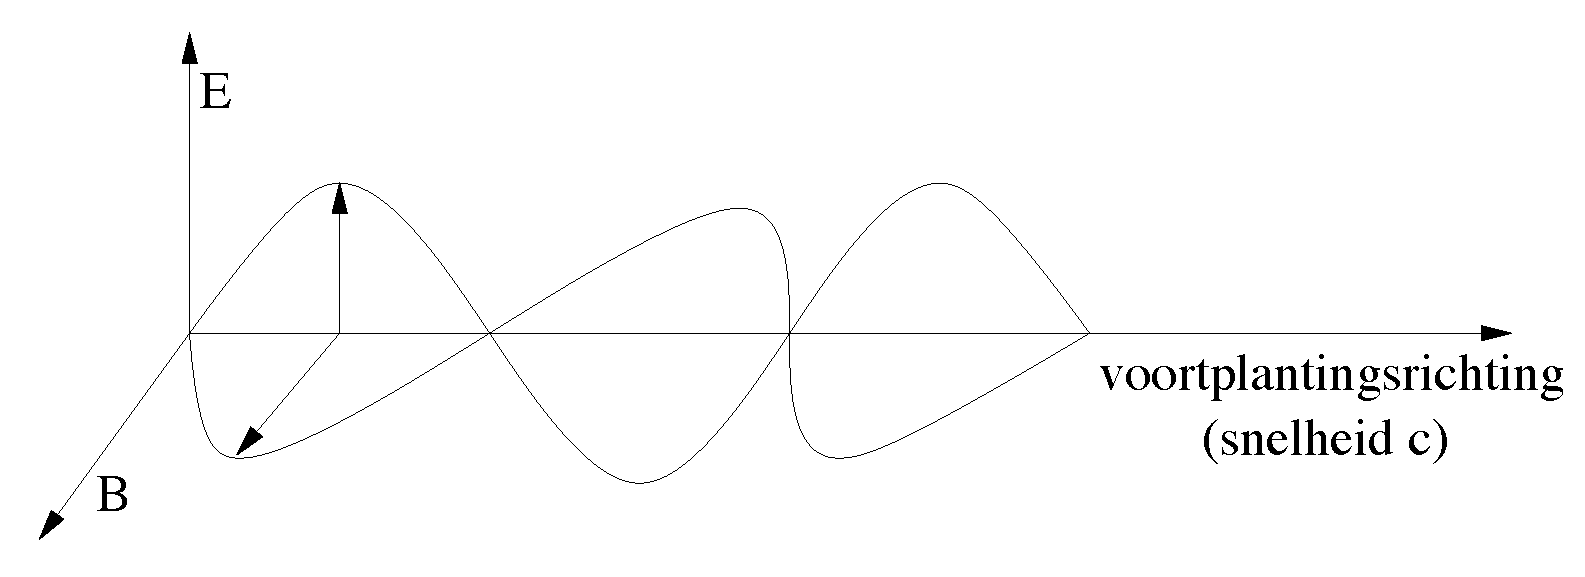
\epsfig{file=emwave.pdf, width=0.7\textwidth}
\caption{{\sl Elektromagnetische golf.}}
\label{f:emgolf1}
\end{figure}

Radiogolven, lichtgolven, R\"{o}ntgenstralen zijn allemaal voorbeelden van 
elektromagnetische golven, allemaal gekarakteriseerd door dezelfde 
voortplantingssnelheid $c$ (waarin verschillen ze?).
De snelheid van het licht in vacu\"um, $c$, is experimenteel exact bepaald op\footnote{Deze waarde defini\"eert de lengte van de meter!}:
\begin{displaymath}
c =  299.792.458  \;\; {\rm m/s} 
\end{displaymath}
\begin{displaymath}
{\rm (ongeveer} \;\; 300.000 \;\; {\rm km/s} = 3 \cdot 10^{8} \;\; {\rm m/s})
\end{displaymath}
De vraag die de natuurkunde zich stelde in de periode v\'{o}\'{o}r
Einstein was: wat is het medium waarin elektromagnetische
golven, zoals lichtgolven, zich bewegen?  Wat golft er nu eigenlijk? 
Het `natuurlijke' co\"{o}rdinatenstelsel om elektromagnetische
verschijnselen te beschrijven is dan het co\"{o}rdinatenstelsel ten
opzichte waarvan dit medium in rust is. Het medium werd als re\"eel
beschouwd, en werd `ether' genoemd.  Zoals Einstein zou laten zien was
dit de verkeerde vraag, de ether bestaat eenvoudigweg niet! 

\subsection{Het Michelson \& Morley-experiment}
Het was Ole Roemer die in 1676 voor het eerst aantoonde dat licht een
eindige snelheid heeft. Hij deduceerde dit door zorgvuldig het
tijdstip bij te houden, waarop de maan Io binnentreedt in de schaduw
van de planeet Jupiter, waar Io in 1,77 dagen omheen loopt.  Door de
situatie tijdens oppositie (waar de aarde tussen zon en Jupiter in
staat) en conjunctie (waar de zon tussen aarde en Jupiter staat - en
we dus Jupiter maar moeizaam kunnen waarnemen) met elkaar te
vergelijken ontdekte Roemer dat er een discrepantie was die verklaard
kon worden door aan te nemen dat het licht er ca. 22 minuten voor
nodig had om de aardbaan te doorkruisen, oftewel een afstand af te
leggen van 2 A.E. (Astronomische Eenheden). Met 1 A.E. de gemiddelde
afstand van de aarde tot de zon, bepaald op ca. 150 miljoen km, kwam
Christiaan Huygens twee jaar later uit op een snelheid van 200.000
km/s.  In feite is de snelheid van het licht ca. 300.000 km/s, zodat
Roemer een systematische fout had (in werkelijkheid heeft het licht 16
\`a 17 minuten nodig om de aardbaan te doorkruisen).  

De eerste serieuze laboratorium-metingen om de snelheid van het licht
te achterhalen stammen uit 1849 en werden uitgevoerd door Fizeau, en
stelde de lichtsnelheid vast op 313.000 m/s.  Ook toonde hij aan dat de
lichtsnelheid in een snelstromende vloeistof, zeg met snelheid $v$ in
de voortplantingsrichting van het licht, {\sl niet} toeneemt tot $c+v$ zoals
op basis van de Galileitransformatie verwacht zou worden.

In een beroemde serie van experimenten in de 19$^{\mathrm{e}}$ eeuw probeerden
Michelson en Morley het bestaan van de ether experimenteel aan te
tonen, door meting van de lichtsnelheid ten opzichte van de ether. De
aarde draait om de zon, dus kan de aarde niet in rust zijn ten
opzichte van dit medium, althans niet gedurende elke dag van het jaar
en waarschijnlijk op geen enkele dag. De beweging van de aarde door de
ether kan gemeten worden door de lichtsnelheid in twee loodrecht op elkaar staande richtingen te vergelijken. 

Stelt u zich namelijk voor dat de hypothese van de ether juist is, d.w.z. er is
een medium ten opzichte waarvan de lichtsnelheid de waarde $c$ heeft,
en dat het relativiteitsprincipe van Einstein {\it niet} juist is. Stel
verder voor dat er een experiment wordt uitgevoerd om de snelheid van
het licht $c_{\oplus}$ op aarde te meten, die met snelheid
$\vec{v}_{\oplus}$ (een vector met lengte $v_{\oplus}$) beweegt ten
opzichte van het medium. Als we de snelheid van het licht meten,
parallel met de snelheid van de aarde $\vec{v}_{\oplus}$, vinden we
$c_{\oplus}=c-v_{\oplus}$ omdat de aarde het licht `achtervolgt'. Als
we de snelheid de andere kant op meten, tegenovergesteld aan de
beweging van de aarde, vinden we daarentegen
$c_{\oplus}=c+v_{\oplus}$. Als we nu de snelheid meten loodrecht op de
beweging, vinden we $c_{\oplus}=\sqrt{c^2-v^2_{\oplus}}$ omdat de
lichtsnelheid de hypotenusa is van een rechthoekige driehoek met
zijden van lengte $c_{\oplus}$ en $v_{\oplus}$. Als de hypothese van het bestaan van de ether correct is, laten deze argumenten zien dat de beweging van de aarde
ten opzichte van de ether gemeten kunnen worden.

\begin{figure}[ht]
\centering
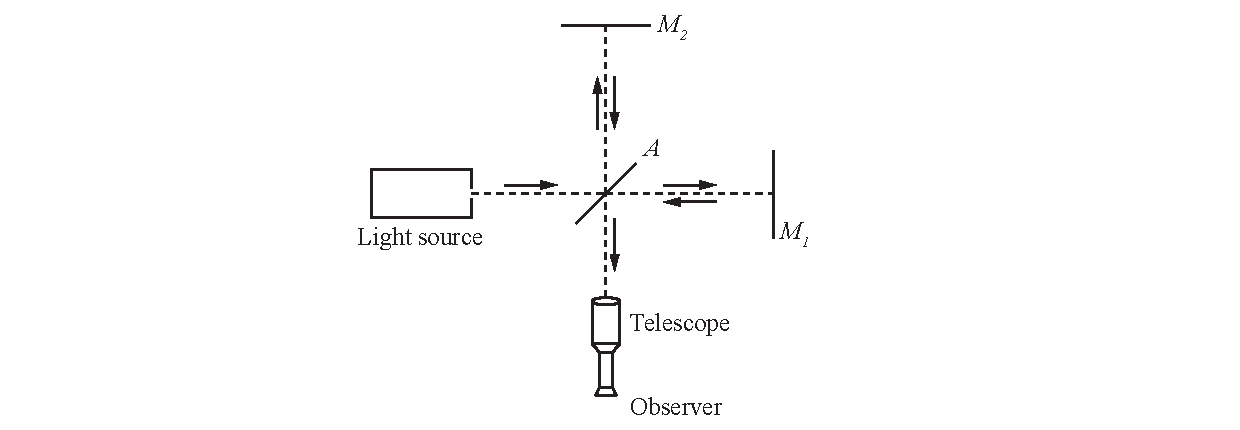
\epsfig{file=MM.pdf, width=\textwidth}
\caption{{\sl Het Michelson \& Morley experiment. Licht uit de `light
source' valt op de halfdoorlaatbare spiegel A. Een gedeelte van het
licht legt het pad via spiegel $M_1$ af, een ander gedeelte een pad
via spiegel $M_2$. In de `telescope' komen de bundels samen en is het interferentiepatroon
zichtbaar.}}
\label{f:mm}
\end{figure}


Het experiment van Michelson \& Morley was ontworpen om deze meting te
verrichten door de lichtsnelheid in twee richtingen loodrecht op elkaar te vergelijken. Omdat het moeilijk is de absolute snelheid te
bepalen, was het experiment ontworpen om de relatieve snelheid van de
twee richtingen te bepalen, met behulp van interferentie van
lichtstralen. In figuur~\ref{f:mm} is het experiment schematisch
weergegeven. Het hele experiment werd gemonteerd op een draaibaar
platform waardoor het gemakkelijk geroteerd kon worden.

Als de totale lengte van elke bundel $l$ is, en een bundel in de
richting parallel met $\vec{v}_{\oplus}$ loopt en de ander daar
loodrecht op, wordt de tijd die het duurt voor het licht om het pad af
te leggen gegeven door:
\begin{equation}
t_{\parallel}=\frac{l}{2(c+v_{\oplus})} +\frac{l}{2(c-v_{\oplus})}
=\frac{lc}{c^2-v^2_{\oplus}}
\end{equation}
omdat de reis van het licht bestaat uit een gedeelte met de stroom mee
en een gedeelte er tegenin. De tijdsduur voor de richting hier
loodrecht op wordt gegeven door
\begin{equation}
t_{\perp} = \frac{l}{\sqrt{c^2-v_{\oplus}^2}}
\end{equation}
omdat deze gehele reis gemaakt wordt loodrecht op de bewegingsrichting. Definieer nu $\beta=v_{\oplus}/c$ en bereken het tijdsverschil tussen de twee paden. We vinden
\begin{equation}
\Delta t = \frac{l}{c}\left[ \frac{1}{1-\beta^2} + \frac{1}{\sqrt{1-\beta^2}}   \right]
\end{equation}
Voor kleine waarden van $x$ geldt $(1+x)^n \sim 1+nx$ en hiermee wordt
\begin{equation}
\Delta t \sim \frac{l}{2c} \beta^2
\end{equation}

Bij een rotatie van het hele apparaat  zal het ene moment de ene arm
parallel aan de bewegingsrichting van de aarde staan, op het andere
moment de andere arm. Bij een draaiing onder een hoek van 90$^o$ wordt het
tijdsverschil tussen de twee armen dus tweemaal $\Delta t$, en dit
verschil moet observeerbaar zijn in het veranderende
interferentiepatroon van de twee lichtbundels. In de opstelling van
Michelson \& Morley zou dit een verschuiving van 0.4 perioden van de
golflengte van het licht moeten opleveren. Echter, er werd geen enkele
verschuiving waargenomen. Ook niet een aantal maanden later, nadat het  experiment is herhaald.

Dit beroemde `nulresultaat' betekende een groot probleem voor de ether
theorie, en leidde tot een aantal speculaties. Bijvoorbeeld, kon het
gebeuren dat de aarde de ether in de baan om de zon `meesleurde'? In
een artikel uit 1904 van Lorentz werd de mogelijkheid geopperd dat
alle bewegende lichamen krimpen in de richting van de beweging, met
een grootte die precies voldoende was om het experimentele
nul-resultaat te verklaren. Al deze idee\"en waren teveel een ad-hoc
oplossing.

De verklaring van Einstein - die zegt dat er helemaal geen ether is en
dat de lichtsnelheid gelijk is voor alle waarnemers - is de verklaring
die stand heeft gehouden. Het Michelson \& Morley experiment was een
poging van de `schipper' om de snelheid van zijn boot te bepalen
zonder uit het raam te kijken of te vergelijken met een ander
voorwerp. Volgens het relativiteitsprincipe waren ze gedoemd te
mislukken.



%%% Local Variables: 
%%% mode: latex
%%% TeX-master: "Galilei"
%%% End: 
